\documentclass[12pt,english,nohyper]{tufte-handout}\usepackage[]{graphicx}\usepackage[]{color}
%% maxwidth is the original width if it is less than linewidth
%% otherwise use linewidth (to make sure the graphics do not exceed the margin)
\makeatletter
\def\maxwidth{ %
  \ifdim\Gin@nat@width>\linewidth
    \linewidth
  \else
    \Gin@nat@width
  \fi
}
\makeatother

\definecolor{fgcolor}{rgb}{0.345, 0.345, 0.345}
\newcommand{\hlnum}[1]{\textcolor[rgb]{0.686,0.059,0.569}{#1}}%
\newcommand{\hlstr}[1]{\textcolor[rgb]{0.192,0.494,0.8}{#1}}%
\newcommand{\hlcom}[1]{\textcolor[rgb]{0.678,0.584,0.686}{\textit{#1}}}%
\newcommand{\hlopt}[1]{\textcolor[rgb]{0,0,0}{#1}}%
\newcommand{\hlstd}[1]{\textcolor[rgb]{0.345,0.345,0.345}{#1}}%
\newcommand{\hlkwa}[1]{\textcolor[rgb]{0.161,0.373,0.58}{\textbf{#1}}}%
\newcommand{\hlkwb}[1]{\textcolor[rgb]{0.69,0.353,0.396}{#1}}%
\newcommand{\hlkwc}[1]{\textcolor[rgb]{0.333,0.667,0.333}{#1}}%
\newcommand{\hlkwd}[1]{\textcolor[rgb]{0.737,0.353,0.396}{\textbf{#1}}}%

\usepackage{framed}
\makeatletter
\newenvironment{kframe}{%
 \def\at@end@of@kframe{}%
 \ifinner\ifhmode%
  \def\at@end@of@kframe{\end{minipage}}%
  \begin{minipage}{\columnwidth}%
 \fi\fi%
 \def\FrameCommand##1{\hskip\@totalleftmargin \hskip-\fboxsep
 \colorbox{shadecolor}{##1}\hskip-\fboxsep
     % There is no \\@totalrightmargin, so:
     \hskip-\linewidth \hskip-\@totalleftmargin \hskip\columnwidth}%
 \MakeFramed {\advance\hsize-\width
   \@totalleftmargin\z@ \linewidth\hsize
   \@setminipage}}%
 {\par\unskip\endMakeFramed%
 \at@end@of@kframe}
\makeatother

\definecolor{shadecolor}{rgb}{.97, .97, .97}
\definecolor{messagecolor}{rgb}{0, 0, 0}
\definecolor{warningcolor}{rgb}{1, 0, 1}
\definecolor{errorcolor}{rgb}{1, 0, 0}
\newenvironment{knitrout}{}{} % an empty environment to be redefined in TeX

\usepackage{alltt}
\usepackage{longtable}
\usepackage{geometry}
\usepackage{tabularx} % Make sure this is in there
\IfFileExists{upquote.sty}{\usepackage{upquote}}{}
\begin{document}



\centerline{\Large\bf This is my Main Title about Diamonds}

\begin{marginfigure}
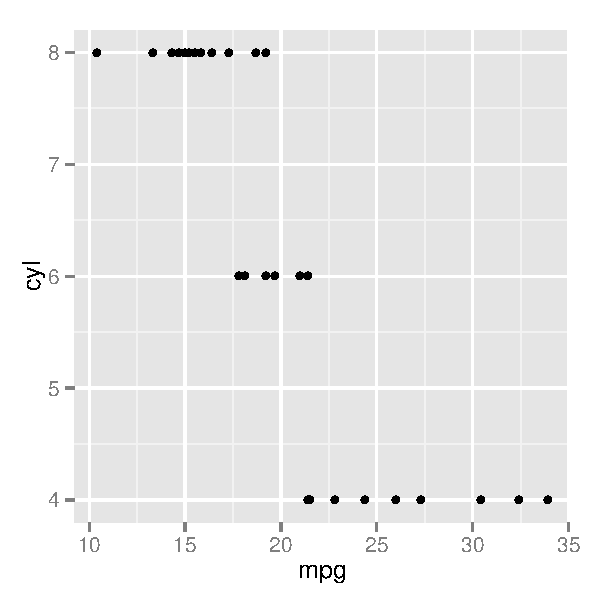
\includegraphics[width=0.98\linewidth]{plot1}
\caption{\label{mar:hist}DEPTH vs PRICE in DIAMONDS dataset.}
\end{marginfigure}

This is the paragraph in my report. This is the paragraph in my report. This is the paragraph in my report. This is the paragraph in my report. This is the paragraph in my report. This is the paragraph in my report. This is the paragraph in my report.

This is the paragraph in my report. This is the paragraph in my report. This is the paragraph in my report. This is the paragraph in my report. This is the paragraph in my report. This is the paragraph in my report. This is the paragraph in my report. This is the paragraph in my report. This is the paragraph in my report. This is the paragraph in my report. This is the paragraph in my report. 

\bigskip{}

\begin{fullwidth}
\makeatletter\setlength\hsize{\@tufte@fullwidth}\makeatother
% latex table generated in R 3.1.3 by xtable 1.7-4 package
% Tue Jul 28 15:44:42 2015
\begin{longtable}{r|lr|r}
  \hline
carat & cut & color & clarity \\ 
  \hline
0.23 & Ideal & E & SI2 \\ 
  0.21 & Premium & E & SI1 \\ 
  0.23 & Good & E & VS1 \\ 
  0.29 & Premium & I & VS2 \\ 
  0.31 & Good & J & SI2 \\ 
  0.24 & Very Good & J & VVS2 \\ 
  0.24 & Very Good & I & VVS1 \\ 
  0.26 & Very Good & H & SI1 \\ 
  0.22 & Fair & E & VS2 \\ 
  0.23 & Very Good & H & VS1 \\ 
  0.30 & Good & J & SI1 \\ 
  0.23 & Ideal & J & VS1 \\ 
  0.22 & Premium & F & SI1 \\ 
  0.31 & Ideal & J & SI2 \\ 
  0.20 & Premium & E & SI2 \\ 
  0.32 & Premium & E & I1 \\ 
  0.30 & Ideal & I & SI2 \\ 
  0.30 & Good & J & SI1 \\ 
  0.30 & Good & J & SI1 \\ 
  0.30 & Very Good & J & SI1 \\ 
  0.30 & Good & I & SI2 \\ 
  0.23 & Very Good & E & VS2 \\ 
  0.23 & Very Good & H & VS1 \\ 
  0.31 & Very Good & J & SI1 \\ 
  0.31 & Very Good & J & SI1 \\ 
  0.23 & Very Good & G & VVS2 \\ 
  0.24 & Premium & I & VS1 \\ 
  0.30 & Very Good & J & VS2 \\ 
  0.23 & Very Good & D & VS2 \\ 
  0.23 & Very Good & F & VS1 \\ 
  0.23 & Very Good & F & VS1 \\ 
  0.23 & Very Good & F & VS1 \\ 
  0.23 & Very Good & E & VS1 \\ 
  0.23 & Very Good & E & VS1 \\ 
  0.23 & Very Good & D & VS1 \\ 
  0.23 & Good & F & VS1 \\ 
  0.23 & Good & E & VS1 \\ 
  0.31 & Good & H & SI1 \\ 
  0.26 & Very Good & D & VS2 \\ 
  0.33 & Ideal & I & SI2 \\ 
  0.33 & Ideal & I & SI2 \\ 
  0.33 & Ideal & J & SI1 \\ 
  0.26 & Good & D & VS2 \\ 
  0.26 & Good & D & VS1 \\ 
  0.32 & Good & H & SI2 \\ 
  0.29 & Premium & F & SI1 \\ 
  0.32 & Very Good & H & SI2 \\ 
  0.32 & Good & H & SI2 \\ 
  0.25 & Very Good & E & VS2 \\ 
  0.29 & Very Good & H & SI2 \\ 
  0.24 & Very Good & F & SI1 \\ 
  0.23 & Ideal & G & VS1 \\ 
  0.32 & Ideal & I & SI1 \\ 
  0.22 & Premium & E & VS2 \\ 
  0.22 & Premium & D & VS2 \\ 
  0.30 & Ideal & I & SI2 \\ 
  0.30 & Premium & J & SI2 \\ 
  0.30 & Very Good & I & SI1 \\ 
  0.30 & Very Good & I & SI1 \\ 
  0.30 & Good & I & SI1 \\ 
  0.35 & Ideal & I & VS1 \\ 
  0.30 & Premium & D & SI1 \\ 
  0.30 & Ideal & D & SI1 \\ 
  0.30 & Ideal & D & SI1 \\ 
  0.42 & Premium & I & SI2 \\ 
  0.28 & Ideal & G & VVS2 \\ 
  0.32 & Ideal & I & VVS1 \\ 
  0.31 & Very Good & G & SI1 \\ 
  0.31 & Premium & G & SI1 \\ 
  0.24 & Premium & E & VVS1 \\ 
  0.24 & Very Good & D & VVS1 \\ 
  0.30 & Very Good & H & SI1 \\ 
  0.30 & Premium & H & SI1 \\ 
  0.30 & Premium & H & SI1 \\ 
  0.30 & Good & H & SI1 \\ 
  0.26 & Very Good & F & VVS2 \\ 
  0.26 & Very Good & E & VVS2 \\ 
  0.26 & Very Good & D & VVS2 \\ 
  0.26 & Very Good & D & VVS2 \\ 
  0.26 & Very Good & E & VVS1 \\ 
  0.26 & Very Good & E & VVS1 \\ 
  0.26 & Very Good & D & VVS1 \\ 
  0.26 & Ideal & E & VVS2 \\ 
  0.38 & Ideal & I & SI2 \\ 
  0.26 & Good & E & VVS1 \\ 
  0.24 & Premium & G & VVS1 \\ 
  0.24 & Premium & H & VVS1 \\ 
  0.24 & Premium & H & VVS1 \\ 
  0.24 & Premium & H & VVS2 \\ 
  0.32 & Premium & I & SI1 \\ 
  0.70 & Ideal & E & SI1 \\ 
  0.86 & Fair & E & SI2 \\ 
  0.70 & Ideal & G & VS2 \\ 
  0.71 & Very Good & E & VS2 \\ 
  0.78 & Very Good & G & SI2 \\ 
  0.70 & Good & E & VS2 \\ 
  0.70 & Good & F & VS1 \\ 
  0.96 & Fair & F & SI2 \\ 
  0.73 & Very Good & E & SI1 \\ 
  0.80 & Premium & H & SI1 \\ 
   \hline
\hline
\caption{Diamonds have an interesting dataset.} 
\label{tab:mtcars}
\end{longtable}

\end{fullwidth}

\end{document}
